\begin{frame}{Fractional divisors}



%\begin{figure}
\begin{equation} \label{pic:M-curve} \notag
% \begin{center}
  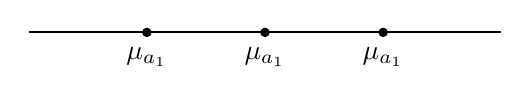
\begin{tikzpicture}
    \draw[thick] (-3,0) -- (3,0);
    % \draw plot[only marks,mark=*] coordinates{(0,0)};
    % \draw plot[only marks,mark=*] coordinates{(-1.5,0)};
    \filldraw[draw=black,fill=black] (-1.5,0) node [below=2pt]
    {$\mu_{a_1}$} circle (1.5pt); \filldraw[draw=black,fill=black] (0,0)
    node [below=2pt] {$\mu_{a_1}$} circle (1.5pt);
    \filldraw[draw=black,fill=black] (1.5,0) node [below=2pt] {$\mu_{a_1}$}
    circle (1.5pt);
    % \filldraw[draw=white,fill=white] (0,-1) node {$\mu_3$} circle
    % (8pt); don't do this
  \end{tikzpicture}
%\end{center}
\end{equation}

\begin{remark}
  \begin{enumerate}
  \item Divisors are now \textbf{fractional}.
  \item $D = D_0 + \frac{n_{1}}{a_!}P_1 + \frac{n_{2}}{a_2}P_2 + \frac{n_{3}}{a_3}P_{3}$
  \end{enumerate}

\end{remark}

\begin{block}{Fact}
  \[
K_{\scrX} = K_X + \sum \frac{e_P-1}{e_P} P
\]
\end{block}


\end{frame}
%%% Local Variables: 
%%% mode: latex
%%% TeX-master: "../ZBVoight-UNC-canonical-stacky"
%%% End: 
